\documentclass[conference]{IEEEtran}
\IEEEoverridecommandlockouts
% The preceding line is only needed to identify funding in the first footnote. If that is unneeded, please comment it out.
\ifCLASSOPTIONcompsoc
 \usepackage[caption=false,font=footnotesize,labelfont=sf,textfont=sf]{subfig}
\else
 \usepackage[caption=false,font=footnotesize]{subfig}
\fi
\usepackage{cite}
\usepackage{amsmath,amssymb,amsfonts}
\usepackage{algorithmic}
\usepackage{graphicx}
\usepackage{textcomp}
\def\BibTeX{{\rm B\kern-.05em{\sc i\kern-.025em b}\kern-.08em
    T\kern-.1667em\lower.7ex\hbox{E}\kern-.125emX}}
\begin{document}

\title{Paper Title*\\
{\footnotesize \textsuperscript{*}Note: Sub-titles are not captured in Xplore and
should not be used}
\thanks{Identify applicable funding agency here. If none, delete this.}
}

\author{\IEEEauthorblockN{Isaac Sacramento}
\IEEEauthorblockA{\textit{Department of Informatic and Statistics} \\
\textit{Federal University of Santa Catarina}\\
Florianópolis, Brazil \\
isaac.sacramento@posgrad.ufsc.br}
\and
\IEEEauthorblockN{Mauro Roisenberg}
\IEEEauthorblockA{\textit{dept. name of organization (of Aff.)} \\
\textit{name of organization (of Aff.)}\\
Florianópolis, Brazil \\
email address}
\and
\IEEEauthorblockN{Rodrigo Exterkoetter}
\IEEEauthorblockA{\textit{Departament of Computer Science} \\
\textit{Federal University of Santa Catarina}\\
Florianópolis, Brazil \\
email address}
\and
\IEEEauthorblockN{Leando P. de Figueiredo}
\IEEEauthorblockA{\textit{Departament of Physics)} \\
\textit{Federal University of Santa Catarina}\\
Florianópolis, Brazil \\
email address}
\and
\IEEEauthorblockN{5\textsuperscript{th} Given Name Surname}
\IEEEauthorblockA{\textit{dept. name of organization (of Aff.)} \\
\textit{name of organization (of Aff.)}\\
City, Country \\
email address}
\and
\IEEEauthorblockN{6\textsuperscript{th} Given Name Surname}
\IEEEauthorblockA{\textit{dept. name of organization (of Aff.)} \\
\textit{name of organization (of Aff.)}\\
City, Country \\
email address}
}

\maketitle

\begin{abstract}
This document is a model and instructions for \LaTeX.
This and the IEEEtran.cls file define the components of your paper [title, text, heads, etc.]. *CRITICAL: Do Not Use Symbols, Special Characters, Footnotes, 
or Math in Paper Title or Abstract.
\end{abstract}

\begin{IEEEkeywords}
component, formatting, style, styling, insert
\end{IEEEkeywords}

\section{Introduction}
Deblurring is the task of estimating a sharp latent image,
given a blurry image as input.
% Recovering the original image
% is possible if the details of the blurring method are known, but
% in most cases, blurry images lack of enough information
% to recover a unique image \cite{}. 
It is not observable in the literature
an algorithm for deblurring all objects. Thus, methods that exploit
domain-specific knowledge have emerged for deblurring
categories of objects, e.g., text, faces and motion images \cite{Grigorios2017}.
In oil exploration field, the seismic data acquisition and its
inversion to acoustic impedance attribute typically generates
blurry images of the subsurface, in such a way that it is not
clearly observe the interfaces between different rock layers,
geological structures such as channels, etc.
Obtaining high resolution acoustic impedance images, through seismic inversion methods,
is a critical part in oil reservoir characterization.
Despite the notorious efficiency of the inversion methods,
post-inversion images deblurring has not received much attention.

%O GAP
Reservoir characterization aims to determine a multidimensional
structure and properties of an oil field. To achieve this goal, it is essential to combine, through an
inversion algorithm, the informations, knowledges and available data about the field,
in such a way that it is possible to make the
quantitative predictions about the reservoir behavior \cite{buiting}.
%One of the data used in this process is the seismic amplitude.
The seismic data is widely used in inversion processes because of its facility and precision
in interpreting the acoustic impedance property.
To succeed in seismic inversion, it is necessary to include strategies to deal with multiple
sources of uncertainties. Specifically, the limited band-width of the seismic data leads to
a misinterpretation of the resulting acoustic impedance models.
According to \cite{xiaoiu}, improving the resolution of seismic inversion is
possible by adding high frequency in acquisition and processing seismic data.
However, the earth attenuation, high-frequency noise and other sources, cause
the lack of high and low frequencies in seismic data. 
Thus, deblurring the acoustic impedance models, as a post-inversion refinement process, should lead to a more accurate
interpretation of the impedance models.

We approach  the acoustic impedance deblurring through
a CNN model. CNN is a framework of deep learning which has been
used in a wide sort of machine learning tasks. The availability of benchmarks
\cite{Russakovsky} and the advances in Graphical Processing Unit (GPU) \cite{Buduma15}
allowed CNN to outperform state-of-the-art techniques in detection \cite{Girshick2015,Bell2015}, model-free
tracking \cite{Nam}, classification \cite{He2016}. With excellence in feature learning,
CNN achieved notorious success in image and video classification \cite{Krizhevsky2012, AbdelHamid2014}, action  and speech recognition \cite{Farfade2015, S_Ji2013}.
Under the perspective of the reservoir characterization, CNN has been applied to lithofacies recognition
\cite{Qian} and calculation \cite{Liu2017}. However, there is a lack of researches on improving the resolution of
images resulting from inversion processes.

%A solução
In this paper, we propose a new multilayer convolution network model to perform deblurring in post-inversion acoustic impedance.
Each network layer maps higher level features originated in the previews layers through convolutional blur kernels.
To perform this mapping, the kernels, also named weights, are adjusted by minimizing a loss function. 
The model enhances the resolution of acoustic impedance images, resulting in sharp images with
increased high-frequency band-width and lower noise. 
In order to train the model, we blur a set of the synthetic acoustic impedance images to create a dictionary of
images of high and low resolution. Then, the pairs of blur and latent images are normalized and 
presented to the network as input and target, respectively.
%We compare the deblurred images depicted by our model and by two other deblurring methods ().
The core concept of our architecture is the combination of the convolution layers with regression
layers, thus the convolutional layers learn the spatial structures existing in different
acoustic impedance images, while the regression layer proceed the prediction of the property values.

\section{Theoretical Foundations and Related Works}
Inversion theory is used in several areas to infer parameters values
related to physical processes based on experimental data.
Inversion modeling refers to using the current measurements of observable
physical parameters in order to infer the current model parameters (not observable).
The inversion problem is described as  \eqref{eq:deqgm}
\begin{equation}
\label{eq:deqgm}
m = F^{-1}(d)
\end{equation}
where, $F$ is the investigated physical system, and relates a set of model parameters
$m=(m_1, m_2,...,m_n)\subset R^n$ estimated through the observed data $d \in R^s$.
Geophysical methods frequently involve the solution and assessment of inversion problems.
Studying these problems allow inferring physical properties distributions in the earth subsurface, using measured
data. Among these data, the seismic data is mainly used in seismic inversion, which plays an important role in
reservoir characterization. From a practical perspective, solving seismic inversion problems improves
the exploration and management in oil industry, once the seismic data is highly correlated to petrophysical
properties, e.g., density and porosity in subsurface.

The offshore seismic data is the main observable data used in seismic inversion. To perform seismic acquisition,
one sends pulses through a controlled artificial source and captures
the vertical component responses in function of time. The seismic data is a composition of
the wave pulse used in the acquisition, named wavelet, and the characteristic of the interfaces between rock layers,
on which the wavelet reflects. This rock layer characteristic is called reflectivity coefficient and it is
calculated as \eqref{eq:refletv}
\begin{equation}
r(t) = \frac{z(t+\delta t)-z(t)}{z(t+\delta t)+z(t)},
\label{eq:refletv}
\end{equation}
where, $z(t)$ is the acoustic impedance, in function of time $t$, defined as 
$z(t)=\rho(t)v(t)$, where $\rho(t)$ is the rock density and $v(t)$ the propagation velocity
of acoustic wave.
Therefore, the seismic data  $d(t)$ is modeled as a discrete convolution operation $*$ of the wavelet $s$ with the
reflectivity coefficient $r$ as \eqref{eq:seismic_conv}
\begin{equation}
d(t) = s(\tau) * \sum_{j-1}^{N}{r(t- t_j) \delta(t - t_j) + e_d(t)}
\label{eq:seismic_conv}
\end{equation}
where, $N$ is the number of subsurface layers, $e_d(t)$ is a random noise in function of time.
One ideal wavelet is a delta pulse with all the frequency band-width, however, in practice
wavelets have their band-width generally limited from $6Hz$ to $65Hz$. By consequence,
the images resulting from the seismic inversion will keep their frequency spectrum limited.

According to \cite{Latimer2017}, a good acoustic impedance model contains more information
than the seismic data, because the inversion process contains additional information originated from well-logs, for
exemple, a low-frequency model.
The well-logs are real data measured in wells spread along the field.
With the local acoustic impedance it is possible to calculate the low-frequency
model by interpolation between wells \cite{Buland2003,Figueiredo2012}. Despite of the
low-frequency model, the final model for acoustic impedance still lacks of high resolution details.

Deblurring is generally modeled as the convolution of a blur kernel $k$
with a latent image $I$: 
\begin{equation}
 y = k \otimes I + n
 \label{eq:deblurr}
\end{equation}
where $n$ is the noise. Since $k$, $I$ and $n$ are unknown, the problem 
is highly ill-posed and admits infinity solutions for $k$ and $I$.
Several works have developed different deblurring methods for specific purposes.
Blind deconvolution methods are widely investigated in image processing \cite{Bishop2007}.
For the last six years, considerable effort has been employed in single image
\cite{Babacan2012,Krishnan2015,Levin2011,Zhang2011} and multi-image \cite{sroubek2012,Zhu2012} blind deconvolutions. 
Applying blind deconvolution generally implies in making assumptions on
blur kernels and/or on latent images. For example, assuming sparsity of blur kernel
or that natural images have super-Gaussian statistics. The second assumption
leads to the use of image priors on inference process and, consequently, to the maximum \textit{a posteriori}
(MAP) estimation \cite{Babacan2012}. However, \cite{Levin} show that deblurring methods
based on this prior tend to favor blurry images over original latent images.
%,specially for algorithms formulated within the MAP framework.

The Bayesian inference approach \cite{Levin} outperforms the MAP based methods. It marginalizes
the image from the optimization step, while estimating the unknown blur.
The authors show that it is possible to define a class of prior image
based on natural image statistics, suitable enough to represent sharp images features.
This prior formulation makes possible to use Bayesian inference in the estimation of the
unknown image and the blur kernel. According to \cite{Hacohen13}, defining a gradient
prior, by itself, is not sufficient to reach a sharp image, instead,
they search in a dataset for a prior that densely correspond to
the blurry image similar to a sharp image. This search is an
iteratively optimization over the correspondence between the images, the kernel and
the sharp image estimation. Although \cite{Pan2014} suggest a generalization
for the method proposed by \cite{Hacohen13}, it still requires a similar reference image,
which is not always available.

The optimization methods previously described use a set of priors based on
generic image statistics or domain-specific priors. It has been demonstrated
that these methods work properly on synthetic blurs. However, newly studies show that they failure
when applied to real world blurry images \cite{Lai2016} and take a severe computational cost \cite{Chakrabarti2016}.
In contrast, the learning-based methods have gained attention with the resumption and recent advances in neural
networks. The adequate hyper-parameter adjustment allows neural network to learn
non-linear function or blur kernels. Thus, deblurring becomes a function of a blurry image $I$
and a set of parameters $p$ as \eqref{eq:deblur}
\begin{equation}
 y = \sigma(I,p)
 \label{eq:deblur}
\end{equation}
Learning-based methods focus on developing a model to learn the function $\sigma$ \cite{Hradis2015}
and to perform non-blind deblurring \cite{Chakrabarti2016}. \cite{Sun2015} learn a convolution neural networks (CNN) to
recognize motion kernels and performs non-blind deconvolution in
dense motion field estimate, in addition, \cite{Hradis2015} minimize regularized $l_2$ 
in order to perform text deblurring.

\section{Data and Methods} \label{DMsection}
\subsection{Acoustic Impedance Inversion}
The experiments described in this paper perform
on a set of synthetic acoustic impedance images. Using synthetic models
to test and parametrize algorithms is a common practice in reservoir characterization \cite{Sergio2016}. It allows studying the
results of the algorithms without external interferences and performing efficient interpretations and assessments. 
According to \cite{Harvey}, wedge shaped models is a straight way to analysis the
seismic model and inversion processes. It reproduces
reservoir contexts such as stratigraphic refinements, edges and channel structures in a realistic manner.

The training set generation occurs in two steps.
The fist step creates a set of wedge shapes represented
by images with size $32$ x $32$. The wedge shapes represent the reservoir and they
randomly vary in width and length. The second step fills the lithology with values of petrophysical properties.
In order to simplify the assessments and conclusions, we fill the lithology structures with constant
reference values of rock densities and compressional velocity observed in the literature \cite{Mavko2009}.
The acoustic impedance is calculated using the density and velocity models and the images in high
resolution model are obtained, as illustrated in  Fig. \ref{fig_lithology}.
\begin{figure}[!t]
\centering
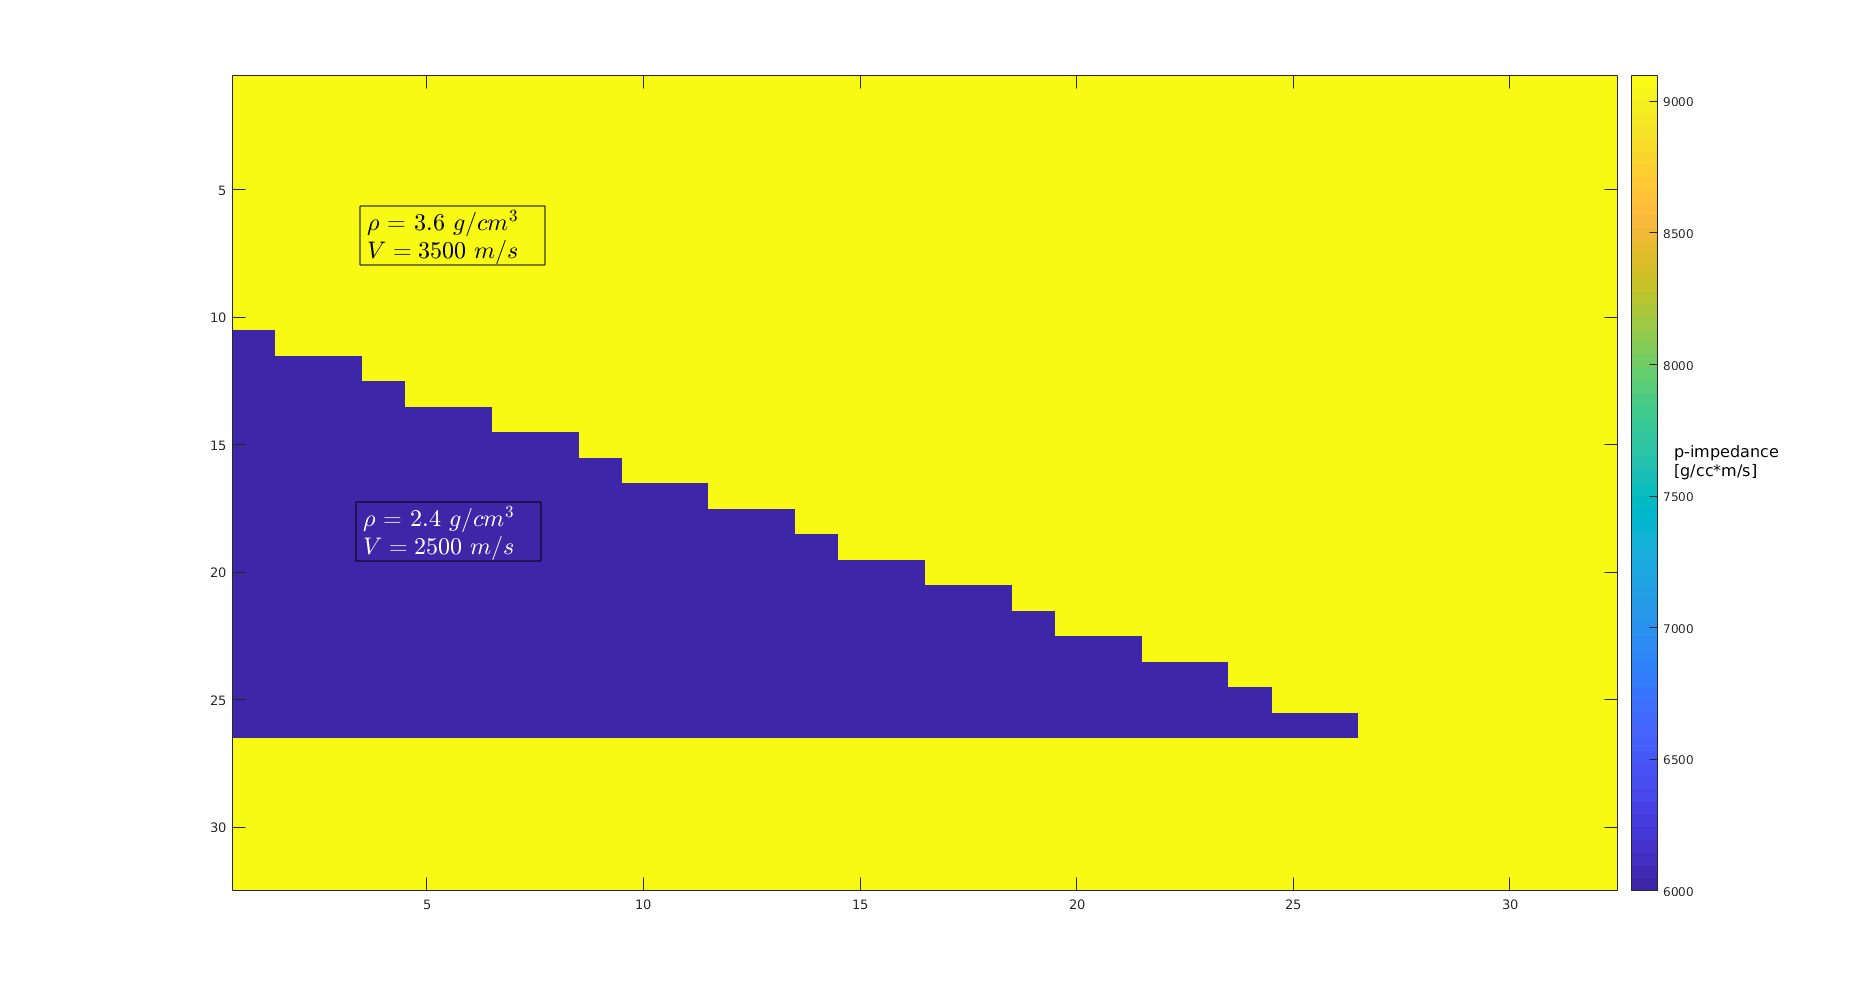
\includegraphics[width=2.0in]{Figs/Image_Paper}
\DeclareGraphicsExtensions.
\caption{Acoustic impedance model generation. Wedge with reference values for density and compressional velocity.}
\label{fig_lithology}
\end{figure}

In a real scenario, the blurry acoustic impedance is the
result of an acoustic inversion method, such as Maximum \textit{a posteriori} \cite{Buland2003,Figueiredo2012}, Sparse Spike \cite{Debeye1990} 
and Recursive Inversion \cite{Chopra2001}, using seismic data with limited band-with.
However, for experimental purpose, the acoustic impedance models were filtered
and the high frequencies were removed to obtain the blurry images, as illustrated in Fig. \ref{fig_blur}.
This way, the supervised learning is performed with the high resolution images and blurred images.
To increase the number of examples in the training dataset we rotate
the impedance models to establish the wedge structure in four different angles
($0^{\circ}$, $90^{\circ}$, $180^{\circ}$ and $270^{\circ}$).
This approach allows the model learning an wide edge variabilities in wedges images.
\begin{figure}[!t]
\centering
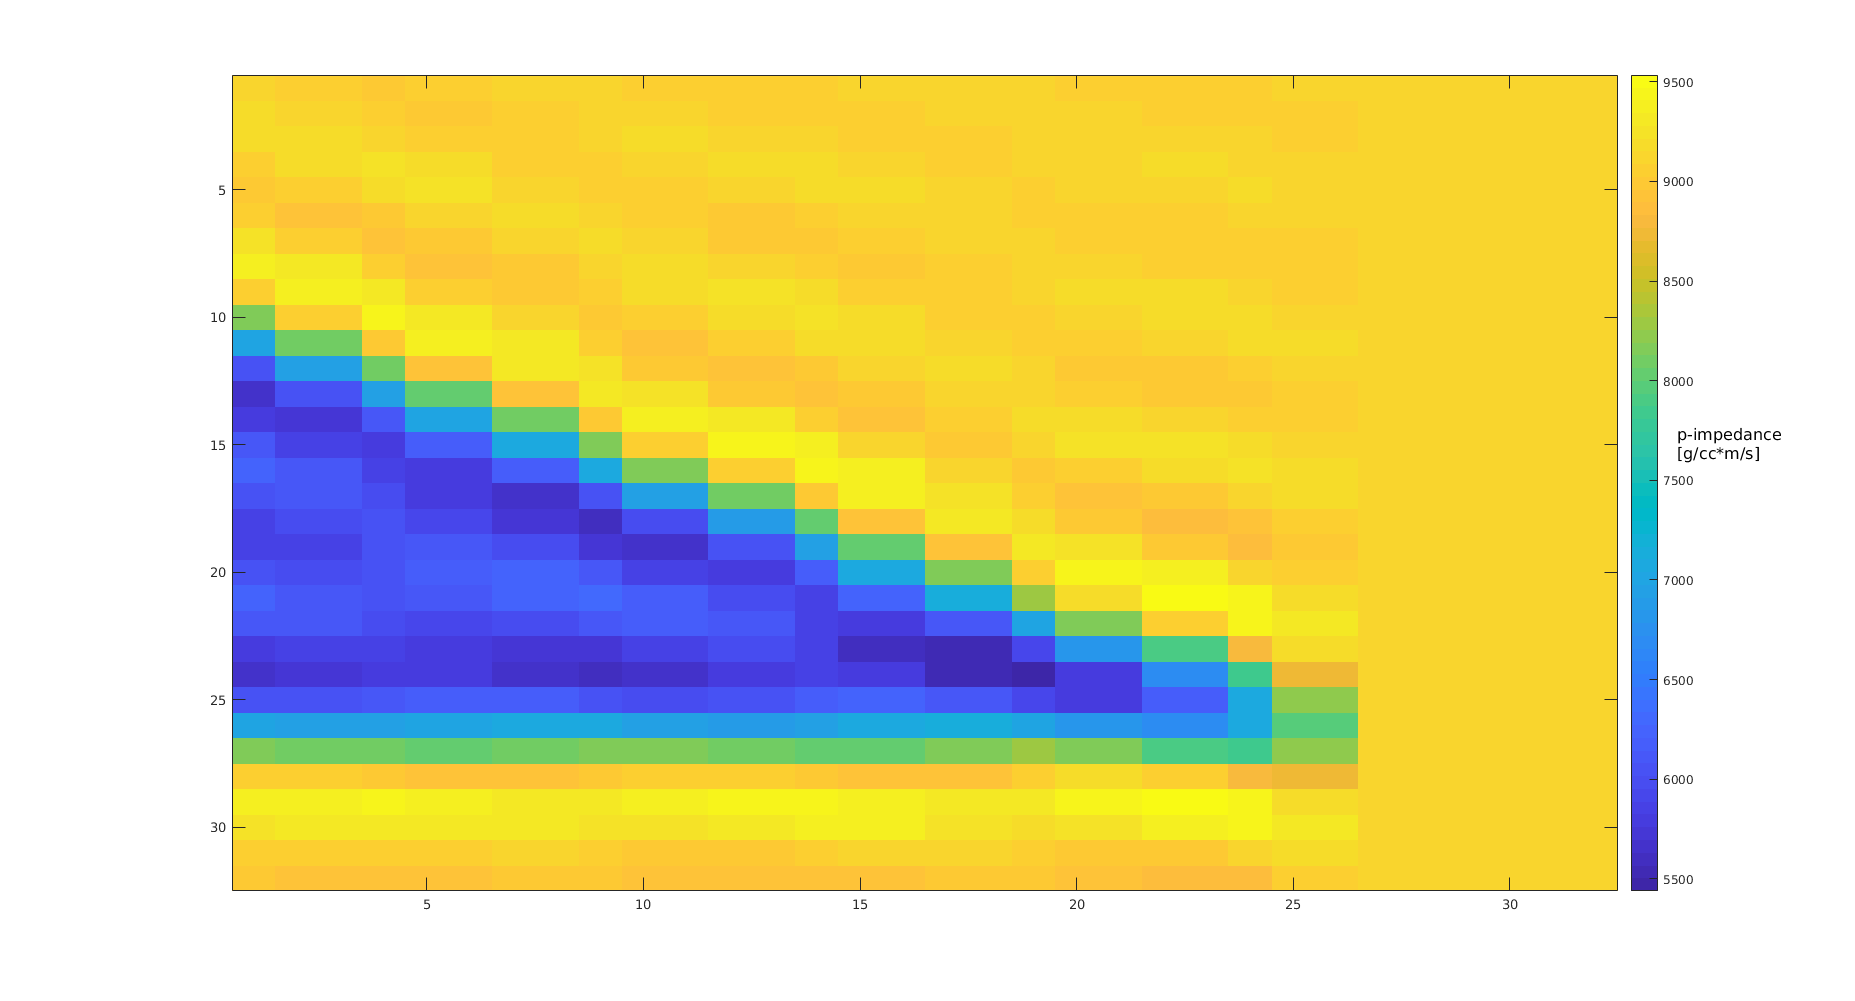
\includegraphics[width=2.0in]{Figs/Image_Paper_blurred}
\DeclareGraphicsExtensions.
\caption{Acoustic impedance blurred model.}
\label{fig_blur}
\end{figure}

\subsection{Proposed Architecture}
The workflow of the proposed method consists of the following
steps:
\begin{itemize}
 \item Generate the synthetic impedance images;
 \item Blur the images through a low-pass filter;
 \item Train the convolutional model with the pair of high and low resolution images;
 \item Test the model with different blurry images;
 \item Assess the result for the testing output.
\end{itemize}

The CNN is a well established method for
pattern recognition and image classification.
Thus, an important breakthrough when applying CNN to
deal with physical property images is developing a model
capable to solve regression tasks. The model presented in this paper
is able to solve two important problems related to deblurring  images of physical properties
: ($1$) learning the spacial patterns in the low resolution
training images and ($2$) predicting each pixel intensity value in the new
higher resolution image. To reach these two goals, our model, outlined in Fig. \ref{fig_model},
% \begin{figure*}[!t]
% \centering
% \subfloat{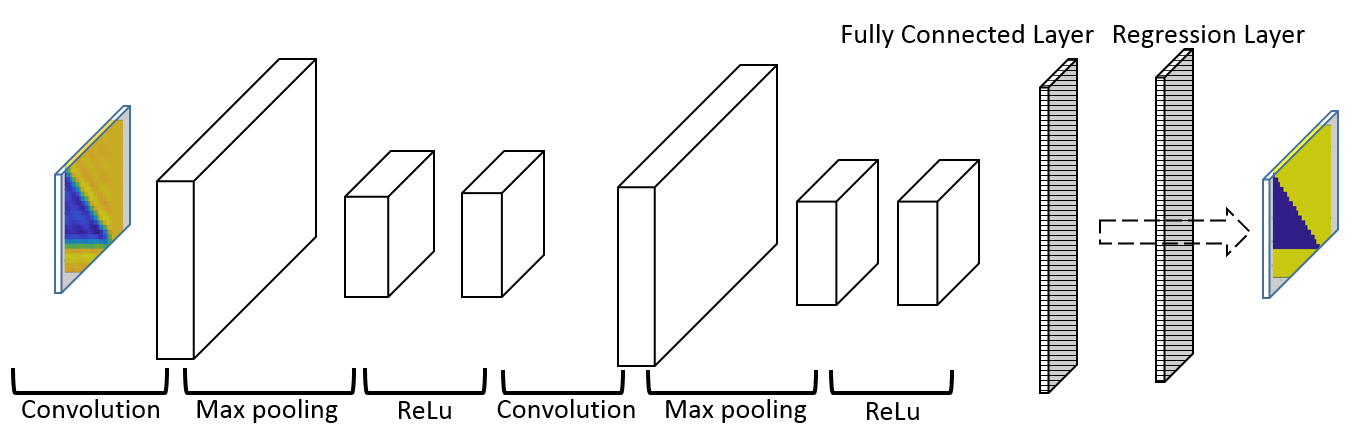
\includegraphics[width=5.0in]{Figs/model}}
% \caption{}
% \label{fig_model}
% \end{figure*}
comprises two major components that are combined to perform deblurring and physical property prediction
jointly: (1) convolutional component and (2) regression component. The convolutional component
is a two layer structure that maps a blurry image to a non-blurred model, while 
the regression layer is supposed to predict the continuous values of each pixel
representing the acoustic impedance value. 
The state-of-the-art CNN models for image deblurring \cite{Grigorios2017} and super-resolution \cite{Dahl2017}
classify each pixel in the input image. 
Using these methods to solve the issue of deblurring continuous physical properties 
implies in discretization of each pixel in order to generate an image file. However, returning
to the original data, results in information loss, what represents a serious inconvenient.
Thus, combining the convolutional approach with the regression layer to deblur and predict
the physics property represents a relevant advance.
\begin{figure}[!t]
\centering
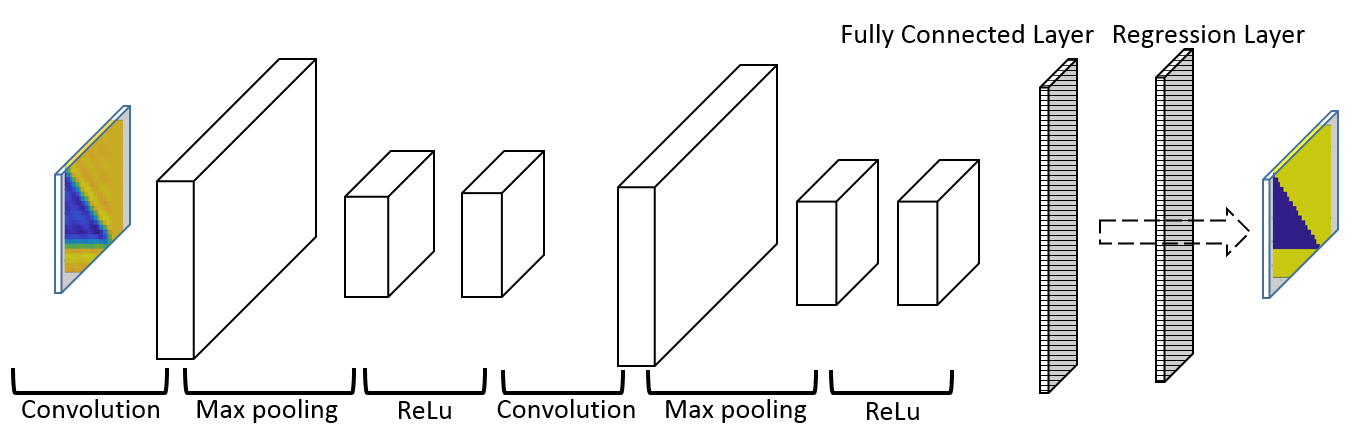
\includegraphics[width=3.0in]{Figs/model}
\DeclareGraphicsExtensions.
\caption{Proposed model achitecture.}
\label{fig_model}
\end{figure}

\subsection{Implementation Details}
The model is implemented using the Deep Learning toolbox
delivered in MATLAB R2017A. Our model comprises a simple architecture with two convolutional layers.
Each one of them is configured with $50$ kernels, sized $5$ x $5$
and stride $1$, meaning that after each convolution operation the blur kernel is shifted
one position in each direction. After each convolutional layer we proceed a maximum pooling operation
to obtain the maximum value of small regions in the input image and obtain  statistical summaries of these regions . We also
apply rectified linear units (ReLU) after each pooling layer in order to speed up the training
step and to learn sensible features from the images, following the proposal of \cite{Nair2010}. After
the second regularization layer,  we add a fully connected layer, which maps the convolution layer's output
to $1024$ neurons. Finally, the output layer comprises a regression unit to predict the intensity of acoustic impedance in each pixel.
The output vector is then resized to the original image dimension.

For training the network, we use a mini-batch with size of $32$ training examples
and we adopt an exponentially decreasing learning rate (initially
set to $0.005$), decreasing every iteration in a total of $100$ iterations.
It should be noted that, once the wedge shapes are randomly generated, every image is different
and each one is introduced only once to the network, this way avoiding over-fitting.
The network weights initialize randomly and the model performs a supervised learning through a dictionary containing pairs of low resolution and high resolution images.
The Stochastic Gradient Descendant with Momentum (SGDM) \cite{Ning1999} adjusts the network weights in every layer by minimizing the Mean Squared Error (MSE)
in each batch of images. Thus, after the training phase, the model is capable
to deblur any other wedge shaped acoustic impedance image not presented in the training dataset. The outputted
image recovers the high frequencies and shows higher similarity
to the high resolution image than to the blurred image, according to a established metric.
The model was adjusted to deblur a wide variety of wedge shapes and impedance values.
Those wedges which the model was unable to predict were added in the training set.

Three metrics assess the performance of the convolution network: Fast Fourier Transform Index - FFTI \eqref{eq:fourier},
Rooted Mean Square Error - RMSE \ref{eq:mse}. 
The FFTI is a similarity metric calculated based on the fast fourier transform (FFT) of each image.
It is introduced by \cite{Naranyana2015} and calculates as 
\begin{equation}
 C = \frac{ (\sum_{i=1}^{N}{F_{1i}F_{2i}} - N \bar{F}_1\bar{F}_2 )^2 }{ (\sum_{i=1}^{N}{|F_{1i}|^2} - N{\bar{F}^2}_1)( \sum_{i=1}^{N}{|F_{2i}|^2} - N{\bar{F}^2}_2 )},
 \label{eq:fourier}
\end{equation}
where, for each frequency, an intensity value is calculated from the real and complex parts of the fourier
transform. $F_{1i}$ represents the intensity value of $i$-th \textit{pixel} in the first image and $F_{2i}$
is the intensity value of $i$-th \textit{pixel} in the second image. $\bar{F}_1$ e $\bar{F}_2$ are the mean
frequencies in each image. The closer FFTI is to $1$, the higher the similarity between the images.
The frequencies spectrum is additionally useful to present the graphic of frequency magnitudes in the images.
The frequency magnitude graphic allows distinguishing what high frequencies were added to the acoustic impedance
after the low resolution image is passed through the trained CNN. 
\begin{equation}
 RMSE = \sqrt{\frac{ (\sum_{i=1}^{N}{(x_i -y_i)^2 } }{N}},
 \label{eq:mse}
\end{equation}

\section{Experiments}
To build the training dataset we generate $500$ images of random wedge.
Because the last layer of the network is a regression unit, it is necessary the
normalization of the images to values between $0$ and $1$, and the results
are presented in terms of this normalization.
The normalized images are then rotated according to the established angles mentioned in Section \ref{DMsection},
then comprising a total of $2000$ images. By doing so, we present to
the network the same lithologies in different positions and expect that the network
identify general sorts of wedges in angles different from those with which the it was trained.
The rotated images are blurred by applying a low-pass filter with
cutting frequency $4Hz$, then the pairs of blurred and not-blurred images are used to
adjust the model weights. It is relevant to mention that the images which are blurred with
the same cutting frequency and that remain symmetric after the rotation, what means that rotating the images causes no changes in impedance values.
In the following subsections we present the results divided into the cases we consider relevant to test. In the
first case, we test the wedges rotated according to the established angles and with acoustic impedance values normalized to $0$ and $1$.
In the second case we invert the impedance values in such a way that the wedges are set with normalized value equal to $1$, and $0$ out of it.
In the third case we test images with impedance values normalized to the interval between $0.3$ and $0.7$, therefore, out of the range used during the training phase.
In the fouth and fith cases we test present to the model wedges rotated at random angles and with random shapes.

\subsection{Integer Angles Rotated Wedges} \label{IARW}
We firstly test if the network is capable to correctly model the shape of the wedges
and to deblur the edges and contours in a simple perspective.
Thus, the training images and the test images have the same reference values for
density and compressional velocity, they are different only by their shapes.
Comparing the blurry image (Fig. \ref{fig_second_case_blurred}) and the CNN output (Fig. \ref{fig_second_case_cnn})
\begin{figure*}[!t]
\centering
\subfloat[Synthetic acoustic impedance images.]{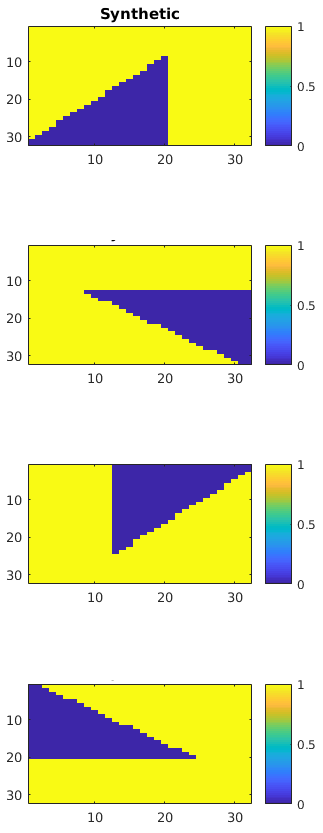
\includegraphics[width=1.5in]{Figs/Caso1/synthetic.png}%
\label{fig_first_case_synthetic}}
\subfloat[Equivalent blurry images.]{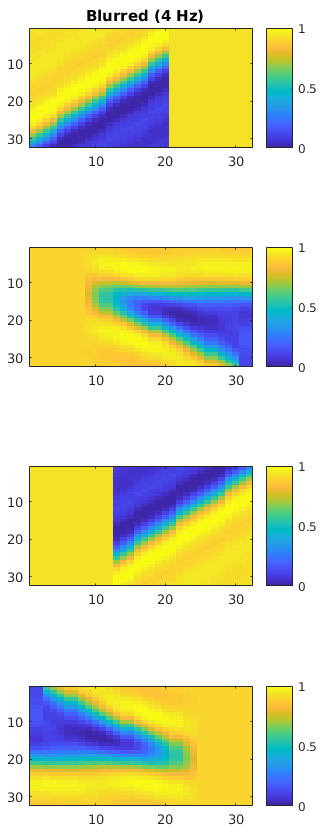
\includegraphics[width=1.5in]{Figs/Caso1/blurred.png}%
\label{fig_second_case_blurred}}
\subfloat[Deblurred acoustic impedance images.]{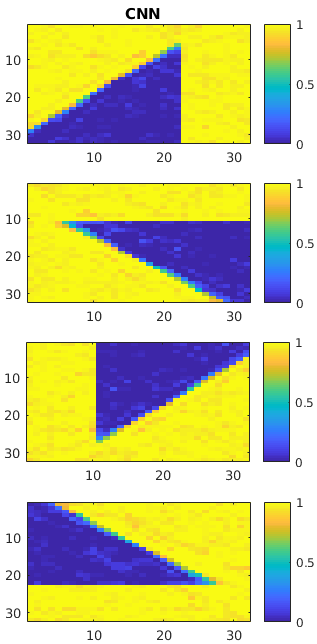
\includegraphics[width=1.5in]{Figs/Caso1/cnn.png}%
\label{fig_second_case_cnn}}
\caption{First test case: the wedges are positioned in 
$0^{\circ}$, $90^{\circ}$, $180^{\circ}$ and $270^{\circ}$ and the acoustic impedance values are normalized to $0$ and $1$.}
\label{fig_scenario1}
\end{figure*}
it is noticeable that the CNN output reached a sharp image and accurately
predicted the pixel values. The RMSE for the network output in Tab. \ref{table_caso_1} is considerably less than the RMSE for the blurry image,
while the FFTI slightly increses and indicates more similarity between the network outputs
and the latent images, except for the first image, for which the IFFT shows not representative change.
The frequency magnitude illustrated in Fig. \ref{fig_frequencies_1}
shows that the model precisely recovered the frequency spectrum of the original image.
\begin{table}[!t]
\renewcommand{\arraystretch}{1.2}
\caption{Metrics values for the first test case.}
\label{table_caso_1}
\centering
\begin{tabular}{|c||c||c|}
\hline
 \textbf{Metrics} & \textbf{\textit{Blurry Image (MSE - FFTI)}} & \textbf{\textit{CNN (MSE - FFTI)}}\\
\hline
Example 1 & $0.1337$ | $0.9773$ & $0.0621$ | $0.9724$\\
\hline
Example 2 & $0.1972$ | $0.9464$ & $0.0776$ | $0.9747$\\
\hline
Example 3 & $0.1337$ | $0.9773$ & $0.0616$ | $0.9861$\\
\hline
Example 4 & $0.1976$ | $0.9498$ & $0.0767$ | $0.9771$\\
\hline
\end{tabular}
\end{table}
% In the second scenario, we invert the impedance values in the lithology structures, that means,
% we fill the reservoir lithology with normalized impedance value equal $1$ and the lithology
% around of the reservoir with value equal to $0$.
% This scenario is absent in the training dataset and we verify independent the convolutional layers and
% the prediction layer work.
% Fig. \ref{fig_scenario6} shows that the model is able to predict the acoustic impedance at any spacial
% position it apears. Similarly to the first test case, the model achieved lower RMSE for the CNN images and higher similarity
% than the blurry images, as seen in Tab. \ref{table_caso_2}.
% Additionaly, in Fig. \ref{} the frequency spectrum recovering is precise in the examples $1$ and $3$. Still, in examples $2$ and $4$ the
% magnitudes of the CNN image are slightly lower than in the synthetic images, for the frequencies above $60Hz$.
% \begin{figure*}[!t]
% \centering
% \subfloat[Synthetic acoustic impedance images.]{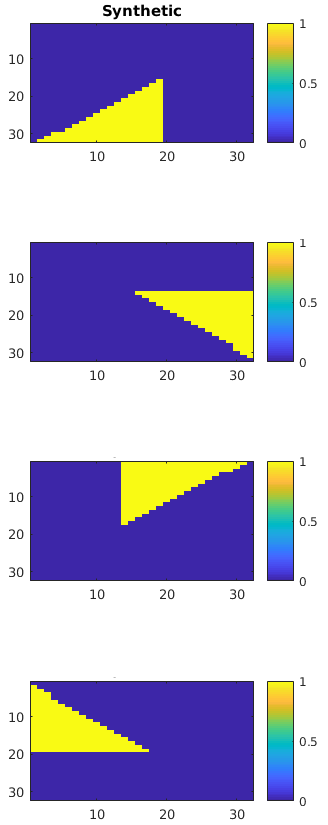
\includegraphics[width=1.5in]{Figs/Caso6/synthetic.png}%
% \label{fig_scenario6_synthetic}}
% \subfloat[Equivalent blurry images]{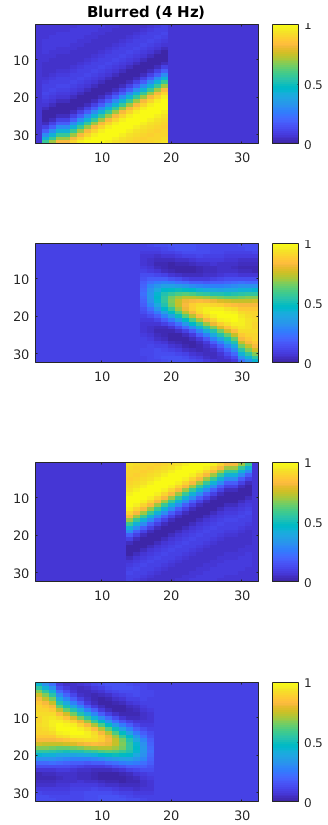
\includegraphics[width=1.5in]{Figs/Caso6/blurred.png}%
% \label{fig_scenario6_blurred}}
% \subfloat[Deblurred acoustic impedance images.]{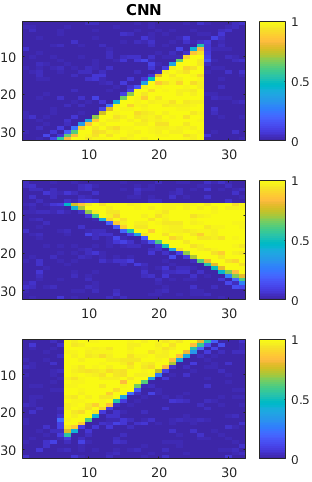
\includegraphics[width=1.5in]{Figs/Caso6/cnn.png}%
% \label{fig_scenario6_case_cnn}}
% \caption{Acoustic impedance models in which the physical property values are inverted in each lithology.
% The wedge are filled with normalized impedance value equal to $1$, while the lithology around the reservoir is filled with values equal to $0$.}
% \label{fig_scenario6}
% \end{figure*}
% 
% \begin{table}[!t]
% \renewcommand{\arraystretch}{1.2}
% \caption{An Example of a Table}
% \label{table_caso_2}
% \centering
% \begin{tabular}{|c||c||c|}
% \hline
%  \textbf{Metrics} & \textbf{\textit{Blurry Image (MSE - FFTI)}} & \textbf{\textit{CNN (MSE - FFTI)}}\\
% \hline
% Example 1 & $0.1294$ | $0.9405$ & $0.0675$ | $0.9416$\\
% \hline
% Example 2 & $0.2033$ | $0.8522$ & $0.0765$ | $0.9046$ \\
% \hline 
% Example 3 & $0.1294$ | $0.9405$ & $0.0701$ | $0.9418$\\
% \hline
% Example 4 & $0.2033$ | $0.8509$ & $0.0763$ | $0.9144$\\
% \hline
% \end{tabular}
% \end{table}

In the following scenario, we arbitrarily change the normalized impedance in both
lithologies to values $ 0.7 $ out of the wedge and $ 0.3$ into the wedge.
These values are different from those first learned by the model during the
training phase and we test the model generalization capacity to reach
the learned pixel intensity values. Once the model is trained with pixel valued to
$ 0 $ and $ 1 $, it poorly extrapolated and a new training dataset is generated containing $30\%$
of the images normalized to the new impedance values. It is noticeable in
Fig. \ref{fig_scenario2} that the network, trained with the new dataset, learned
the wedges shapes and the predicted pixel intensities with low variance. The values
for each image example in Tab. \ref{table_caso_3} show a short decreasing in the RMSE
of the CNN images, while the FTTI indicates a considerable increase in CNN images similarity with the latent image.
Although the short positive change in the metrics, the output images present increasing
frequency magnitude in the range between $ 20 $ and $ 50 Hz $ and between $ 60 $ and $ 100 Hz $.
\begin{figure*}[!t]
\centering
\subfloat[Synthetic acoustic impedance images.]{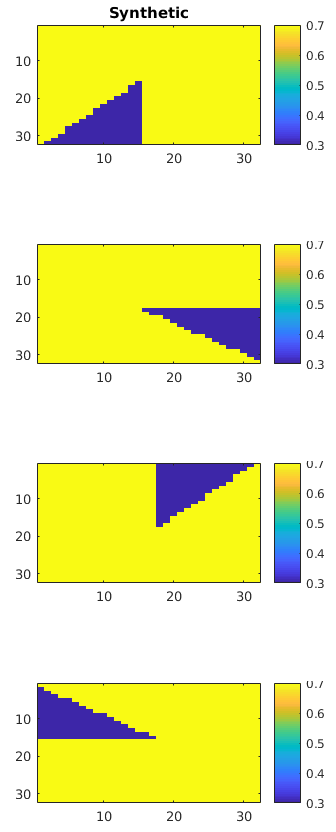
\includegraphics[width=1.5in]{Figs/Caso2/synthetic.png}%
\label{fig_scenario2_synthetic}}
\subfloat[Proposed blurry images filtered with cutting frequency in $4Hz$]{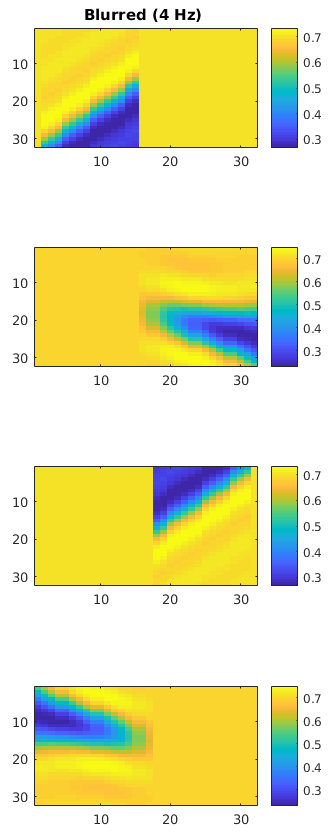
\includegraphics[width=1.5in]{Figs/Caso2/blurred.png}%
\label{fig_scenario2_blurred}}
\subfloat[Deblurred acoustic impedance images.]{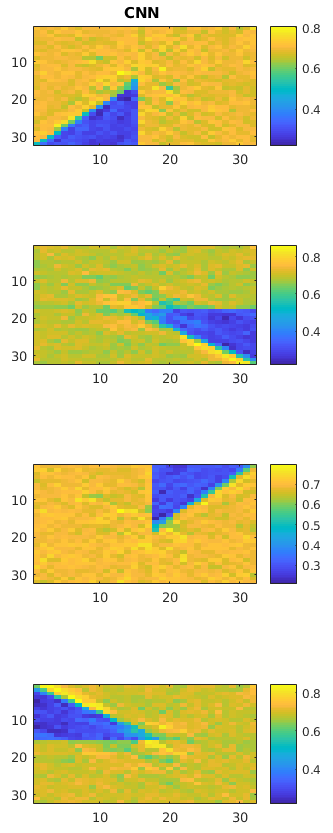
\includegraphics[width=1.5in]{Figs/Caso2/cnn.png}%
\label{fig_scenario2_cnn}}
\caption{The wedges are positioned in $0^{\circ}$, $90^{\circ}$, $180^{\circ}$ and $270^{\circ}$. The acoustic impedance values are normalized to $0.3$ and $0.7$.}
\label{fig_scenario2}
\end{figure*}

\begin{table}[!t]
\renewcommand{\arraystretch}{1.2}
\caption{An Example of a Table}
\label{table_caso_3}
\centering
\begin{tabular}{|c||c||c|}
\hline
 & Blurry Image (MSE - FFTI) & CNN (MSE - FFTI)\\
\hline
Example 1 & $0.0433$ | $0.9830$ & $0.0329$ | $0.0988$\\
\hline
Example 2 & $0.0605$ | $0.9647$ & $0.03677$ | $0.9814$ \\
\hline
Example 3 & $0.0433$ | $0.9830$ & $0.0336$ | $0.9801$\\
\hline
Example 4 & $0.0605$ | $0.9649$ & $0.0374$ | $0.9804$\\ 
\hline
\end{tabular}
\end{table}

\subsection{Randomly Rotated Wedges}
The randomly rotated wedges are related to lithologies positioned at random angles.
In this case, we evaluate the CNN capability to deblur the wedges with specific shape and
position, that are absent of the training dataset.
We test the wedges with the acoustic impedance normalized to values equals to $0$ and $1$.
It is observable in Fig. \ref{fig_scenario4} that the model presents higher uncertainty
in modeling the edges and corners of the wedges. On the other side, as the test images contain the same range of values
as in the training images, the model keep its predictive capacity and recover the  This result is evident in the metrics values
(Tab. \ref{table_caso_6}). In examples $2$ and $4$, the network outputs present lower RMSE than the blurry images, 
while it is higher in the other examples $1$ and $3$. However, according to the FFTI, all the network outputs present
less similarity to the latent image, than the blurred image and we believe that is explained by the higher uncertainty
observed. A mitigation for this problem is adding examples of this image to the network dataset, as stated previously in
Section \ref{IARW}.



\section{Conclusion}

\begin{thebibliography}{00}

\bibitem{Grigorios2017}		G. G. Chrysos, and S. Zafeiriou, ``Deep Face Deblurring.'' pp. 2015-2024, 10.1109/CVPRW.2017.252, 2017. 
\bibitem{buiting} 		JJM. Buiting, M. Bacon,``Using geophysical, geological, and petrophysical data to characterize reservoirs in the North Sea.'' in 5th Conference on Petroleum Geology of NW Europe, London. CD-ROM.
\bibitem{xiaoiu}  		X. Xiaoyu, L. Yun, S. Desheng, G. Xiangyu, and W. Huifeng, ``Studying the effect of expanding low or high frequency on post-stack seismic inversion,'' in SEG Technical Program Expanded Abstracts 2012, pp. 1-5, September 2012.
\bibitem{Russakovsky}		O. Russakovsky, J. Deng, H. Su, J. Krause, S. Satheesh, S. Ma, Z. Huang, A. Karpathy, A. Khosla, M. Bernstein, ``Imagenet large scale visual recognition challenge,'' in ternational Journal of Computer Vision (IJCV), pp. 211–252, 2015.
\bibitem{Buduma15}  		N. Buduma, `` Fundamentals of Deep Learning,'' Academic Press, in O'Reilly Media, 2015.
\bibitem{Girshick2015}		R. Girshick, ``Fast r-cnn,'' In IEEE Proceedings of International Conference on Computer Vision (ICCV), pp. 1440–1448, 2015.
\bibitem{Bell2015}		S. Bell, C. L. Zitnick, K. Bala, and R. Girshick, ``Inside-outside net: Detecting objects in context with skip pooling and recurrent neural networks,'' in arXiv preprint arXiv:1512.04143, 2015.
\bibitem{Nam}			H. Nam and B. Han, ``Learning multi-domain convolutional neural networks for visual tracking,'' In IEEE Proceedings of International Conference on Computer Vision and Pattern Recognition (CVPR) IEEE, 2016.
\bibitem{He2016}		K. He, X. Zhang, S. Ren, and J. Sun, ``Deep residual learning for image recognition,'' In IEEE Proceedings of International Conference on Computer Vision and Pattern Recognition (CVPR). IEEE, 2016.
\bibitem{Krizhevsky2012}	A. Krizhevsky, I. Sutskever, G. E. Hinton, ``Imagenet classification with deep convolutional neural networks: Advances in neural information processing systems,'' 2012, pp. 1097–1105.
\bibitem{AbdelHamid2014}	O. Abdel-Hamid, A.-r. Mohamed, H. Jiang, L. Deng, G. Penn, and D. Yu, ``Convolutional neural networks for speech recognition,'' in IEEE/ACM Transactions on audio, speech, and language processing, num. 22, pp. 1533–1545, 2014.
\bibitem{Farfade2015}		S. S. Farfade, M. J. Saberian, and L.-J. Li, 2015, ``Multi-view face detection using deep convolutional neural networks,'' in Proceedings of the 5th ACM on International Conference on Multimedia Retrieval, ACM, pp. 643–650.
\bibitem{S_Ji2013}		S. Ji,W. Xu, M. Yang, K. Yu, 2013, ``3d convolutional neural networks for human action recognition,'' in IEEE transactions on pattern analysis and machine intelligence, num. 35, p. 221–231.
\bibitem{Qian}			Q. Feng, Y. Miao, S. Ming-Jun, W. Yaojun, H. Guangmin, ``Seismic facies recognition based on prestack data using deep convolutional autoencoder,''.
\bibitem{Liu2017} 			L. Lihui, L. Rong, L. Jianhai, Y. Wenkui, ``Seismic Lithofacies Computation Method Based on Deep Learning,'' in International Geophysical Conference, pp. 649-652, April 2017.
\bibitem{Latimer2017} 		R. B. Latimer, R. Davidson, P. van Riel, ``An interpreter's guide to understanding and working with seismic-derived acoustic impedance data,'' in The Leading Edge, pp. 242-256, vol. 19, num. 3, 2017.
\bibitem{Buland2003}		A. Buland,  and H. Omre, ``Bayesian linearized avo inversion,'' In Geophysics, 2003, pp. 185–198.
\bibitem{Figueiredo2012}	L. P. Figueiredo, M. Santos, M. Roisenberg, G. Neto, and W. Figueiredo, ``Bayesian framework to wavelet estimation and linearized acoustic inversion,'' in Geoscience and Remote Sensing Letters, pp. 1–5, 2012.
\bibitem{Bishop2007}		T.E. Bishop, S.D. Babacan, Amizic, T. Chan, R. Molina, and A. Katsaggelos, ``Blind image deconvolution: problem formulation and existing approaches.'' in. Blindimage deconvolution: theory and applications,  CRC press, 2007.
\bibitem{Babacan2012}		S. D. Babacan, R. Molina, M. N. Do, and A. K. Katsaggelos, ``Bayesian blind deconvolution with general sparse image priors.'' in Proceedings of European Conference on Computer Vision (ECCV), pp. 341–355, 2012.
\bibitem{Krishnan2015}		D. Krishnan, T. Tay, and R. Fergus, ``Blind deconvolution using anormalized sparsity measure.'' In CVPR, 2011.
\bibitem{Levin2011}		A. Levin, Y. Weiss, F. Durand, and W. T. Freeman. ``Efficient marginal likelihood optimization in blind deconvolution.'' In CVPR, 2011.
\bibitem{Zhang2011}		H. Zhang, J. Yang, Y. Zhang, N. M. Nasrabadi, and T. S. Huang, ``Close the loop: Joint blind image restoration and recognition with sparse representation prior.'' in ICCV, 2011. 
\bibitem{sroubek2012}		F. Šroubek and P. Milanfar, ``Robust multichannel blind deconvolution via fast alternating minimization.'' in IEEE Trans. on Image Processing, pp. 1687–1700, 2012.
\bibitem{Zhu2012}		X. Zhu, F. Šroubek, P. Milanfar, ``Deconvolving PSFs for a better motion deblurring using multiple images.'' in ECCV, 2012.
\bibitem{Levin}			A. Levin, Y. Weiss, F. Durand, and W. T. Freeman. ``Understanding and evaluating blind deconvolution algorithms.'' In IEEE Proceedings of International Conference on Computer Vision and Pattern Recognition (CVPR), pp. 1964–1971.
\bibitem{Hacohen13}		Y. Hacohen, E. Shechtman, and D. Lischinski, ``Deblurring by example using dense correspondence.'' In IEEE Proceedings of International Conference on Computer Vision (ICCV), pp. 2384–2391, 2013.
\bibitem{Pan2014}		J. Pan, Z. Hu, Z. Su, and M. H. Yang, ``Deblurring face images with exemplars.'' In Proceedings of European Conference on Computer Vision (ECCV), pp. 47–62. Springer, 2014.
\bibitem{Lai2016}		W.S. Lai, J. B. Huang, Z. Hu, N. Ahuja, and M. H. Yang, ``A comparative study for single image blind deblurring.'' In IEEE Proceedings of International Conference on Computer Vision and Pattern Recognition (CVPR). IEEE, 2016.
\bibitem{Chakrabarti2016}	A. Chakrabarti, ``A neural approach to blind motion deblurring.'' In Proceedings of European Conference on Computer Vision (ECCV), pp. 221–235. Springer, 2016.
\bibitem{Hradis2015}		M. Hradiš, J. Kotera, P. Zemcı́k, and F. Šroubek, ``Convolutional neural networks for direct text deblurring.'' In Proceedings of British Machine Vision Conference (BMVC), 2015.
\bibitem{Sun2015}		J. Sun, W. Cao, Z. Xu, and J. Ponce, ``Learning a convolutional neural network for non-uniform motion blur removal.'' In IEEE Proceedings of International Conference on Computer Vision and Pattern Recognition (CVPR), pp. 769–777, 2015.
\bibitem{Sergio2016}		S. S. Sancevero, A. Z. Remacre, R. S. Portugal, ``O papel da inversão para a impedância no processo de caracterização sísmica de reservatórios.'' in Revista Brasileira de Geofísica, p. 495-512, v. 24, 2006.
\bibitem{Harvey} 		P. J. Harvey, and D. J. MacDONALD, ``Seismic modelling of porosity within the jurassic aged carbonate bank, offshore Nova Scotia,'' in  Canadian Journal of Exploration Geophysics, num. 26, pp. 54–71.
\bibitem{Mavko2009}		G. Mavko, T. Mukerji, and J. Dvorkin, ``The Rock Physics Handbook: Tools for Seismic Analysis of Porous Media.'' Cambridge: Cambridge University Press, pp. 359-369, 2009.
\bibitem{Debeye1990}		H. DEBEYE, and P. RIEL van, ``Lp-norm deconvolution.'' 1990, Geophysical Prospecting, pp. 381–403
\bibitem{Chopra2001}		S. Chopra, ``Integrating coherence cube imaging and seismic inversion.'' The Leading Edge, pp. 354–362, 2001.
\bibitem{Dahl2017}		R. Dahl, M. Norouzi, and J. Shlens, ``Pixel recursive super resolution'' CoRR, 2017.
\bibitem{Nair2010} 		V. Nair, and G. E. Hinton. ``Rectified linear units improve restricted boltzmann machines.'' In Proc. 27th International Conference on Machine Learning, 2010.
\bibitem{Ning1999}		N. Qian, ``On the momentum term in gradient descent learning algorithms,'' in Neural Networks, vol. 12, pp. 145-151, 1999.
\bibitem{Naranyana2015}		S. Narayana, and P. K. Thirivikraman, ``Image similarity using fourier transform,'' in International Journal of Computer Engeneering and Technology, 2015, num. 6, pp. 29–37.
%\bibitem{riel} 			P. van Riel,  ``The past, present and future of quantitative reservoir characterization.'' in The Leading Edge, 19, pp. 878–881.

\end{thebibliography}

\end{document}
